\documentclass[12pt]{article}
\usepackage{mathtools, amsmath, amsfonts, amssymb, siunitx,array}
\usepackage{hyperref, graphicx, wrapfig, geometry}
\usepackage[makeroom]{cancel}
\usepackage{placeins}
\usepackage{float}


\newgeometry{margin=2cm}

\title{Microprocessor Systems - Project Lab Report}
\author{Auguste Lalande, Felix Dube, Juan Morency Trudel}
\date{\today}

\begin{document}
\maketitle
\clearpage

\tableofcontents
\clearpage

\section{Abstract}

\section{Problem Statement}
This project consisted in establishing full duplex communication between a cellphone and an embedded system through Bluetooth. For this purpose, an STM32F407 micro controller mounted on an STMF4Discovery PCB is to be used on the embedded side to gather information from sensors and control LEDS. Furthermore,  the STM32F4xx Cube HAL drivers are to be used to facilitate software development. On the cellphone side, an Android device is to be used for the user interface. Since the STMF4Discovery board is not equipped with any bluetooth functionalities, an intermediate STM32F401RE Nucleo Board with a DB04A1 BLE Shield is to be used. The functionalities to be implemented are listed below:

\begin{enumerate}
\item Temperature monitoring of the STM32F407 micro controller on the android device
\item 3D filtered accelerometer values from the Discovery board to the android device
\item Double tap on the discovery board to wake up the phone
\item Control over 4 LED on the Discovery board from the phone.
\item A user interface on an android application must be developed for efficient visualization of the sensor readings as well as flexible control over the LEDs. 
\end{enumerate}
\section{Theory and Hypothesis}
\subsection{Pulse Width Modulation}
Pulse Width Modulation (PWM) is a modulation technique that allows the control of the power transferred to a load. As the name states, it consist in using a high switching frequency (much higher than what would affect the load) to control the length of pulses and the time period between them. PWM can be used to control brightness of an LED by letting current flow only a certain percentage of a time period. This percentage is called the duty cycle. If the complete cycle frequency is much faster our eyes can perceive, then no flickering is perceivable and the LED simply appears dimmer. Thus, the duty cycle allows the precise control over the brightness of an LED. 
\subsection{Double Tap Feature}
Double tap was a recently introduced on the android platform to wake up cellphones without any hardware button by simply double tapping on the screen. The only sensor required for this feature is an 3D accelerometer. Taps can easily be detected as spikes in the raw value of the acceleration input. By filtering out low frequency noise from other movements, a tap can be detected without any false positives. controlling the delay between taps and other timing parameters can also help improve the filtering of taps. With the right filtering algorithm even light double taps can be detected and this with minimum ressources. 
\subsection{SPI Communication}
The serial peripheral interface (SPI) protocol is a four wire, full duplex, serial interface specification ideal for short range communication between embedded devices. As seen in figure \ref{fig:spi}, the implementation uses two data lines, one clock line, and one slave select line. The data lines are divided into the master in slave out (MISO) which is driven my the slave and the master out slave in (MOSI) which is driven by the master. All communication is synced to the master's clock which is set on the clock line (SCLK). Finally the slave select line (SSL) is used by the master to indicate which slave it is communicating with. In the case where there is only one slave the line can be kept permanently high.

\begin{figure}[!htb]
  \centering
  \includegraphics[scale=0.65]{images/spi.png}
  \caption{SPI Communication Overview}
  \label{fig:spi}
 \end{figure}

\subsection{Bluetooth Low Energy}
Bluetooth Low Energy allows the wireless communication between different devices. The Generic Attribute Profile (GATT) is the protocol used to exchange data over BLE connection. First of all, GATT defines the different roles that the connected devices can adopt. On one hand, a device can be Client. In this role, the device sends request to a server and receives responses from it. On the other hand, a device can be a Server. In this role, the device receives and sends responses to the clients. It is also repsonsable for storing and making the data available to the client.

Moreover, GATT uses the Attribute Protocol (ATT) as its transport protocol. The ATT defines how the data is organised. In the GATT server data are seperated in different section called services. Each services holds one to many characteristics, and these characteristics are what contains the user data. Figure \ref{fig:gatt} illustrate the data structure instroduced by GATT.

\begin{figure}[!htb]
 \centering
 \includegraphics[scale=0.65]{images/GATT.png}
 \caption{GATT Server Overview}
 \label{fig:gatt}
\end{figure}

Each characteristics can have different properties. A characteristic can have Read property, which means that a client can read the data that it contains. It can also have Write property where the user can modify the data that the characteristic holds. Moreover, a characteristic can have the notify property, which allow the server to do a notification operation on it.

\subsection{Android}
An Android phone is a good device to use as a user interface since the view can be change for each application. It also allow to communicate with other devices using many different wireless communication protocol, including BLE which was used for this lab. Additionally, Android application can be easily build using Android Studio.

\section{Implementation}
The implementation of the software on the discovery board was done by recycling the concepts used in previous experiments (\cite{Lab2report}, \cite{Lab4report}) A multi thread operating system was used to simplify The reader can refer to previous

\subsection{LED control}
Four LEDs were used on the nucleo board for feedback. These were hardwired to PWM compliant ports on the microcontroller. Three active LED modes were implemented and can be chosen from the android application:
\begin{enumerate}
\item All 4 LEDs on mode
\item All 4 LEDs off mode
\item Rotating mode where the LEDs take turn being lit in a rotating manner. The speed and direction of the rotation can also be controlled from the Android side. 
\end{enumerate}
Independent to the mode selected, the brightness of each LED could be tuned by the use of PWM. A hardware timer at 10 MHz frequency was used for the control of the PWM. By controlling the duty cycle with the timer, precise regulation of the brightness was achieved.
\subsection{Double Tap (DT) wake up}
Th DT feature was successfully implemented to notify the android device if a double tap was detected. Important filtering was necessary to avoid triggering DT by simply moving the discovery board. The FSM diagram presented in figure \ref{fig:FSMDT} in the appendix gives an overview of the different methods used. To understand why filtering was implemented this way, please refer to the testing section. The acceleromter used for this feature was calibrated using the method from \cite{Lab4report}. The raw values of the accelerometer were used for this algorithm as opposed to the filtered values from the kalman filter described in \cite{Lab2report} to detect spikes. First the algorithm waited for the acceleration value to have an increase followed by a major decrease or vice versa and recorded this as a spike. The amplitude of the increase or decrease was set to 10 mg for detection of the smallest taps. Then a small delay of 20 ms was introduced as a relaxation time for the accelerometer to settle down to avoid reading multiple spikes from one tap. In the following time period of 40 ms, no spikes are to be detected otherwise the first tap is not counted. This acts as a mechanism to avoid DT detection from vibration. If 40 ms pass without any other variation, the spike is recorded as a clean spike. The algorithm then waits for a second tap the same way it did for the first one. If a second clean tap is not detected before 250 ms, then the algorithm starts over by waiting for a first tap.
The resulting DT detection was very accurate and could consistently detect small double taps even on the table on which the discovery board was placed. False positives from sliding the board on the table or from moving the board in the air were rare, happening less than 1\% of the time.
Double tap was implemented independently for x,y and z detection using this technique, except for the fact that when the second tap was not in the same direction as the first one, it was not considered a double tap.

Refer to the code or the FSM ( figure \ref{fig:FSMDT}) for more detailed information on our algorithm.
\subsection{SPI Communication}
SPI communication was used to transfer data between the discovery board and the Nucleo board. It was important for the two boards to be able to communicate because only the Nucleo board was equipped with Bluetooth capabilities while the discovery board was used to acquire data.
 
Although HAL drivers were available which already implemented SPI communication, these were found to be difficult to use. Therefore the communication was implemented without the use of said drivers. A simple protocol was implemented whereby the Nucleo board would wait for a START\_BYTE indicating the beginning of communication, after which all data was transferred between the boards one byte at a time. In the case where the data to be communicated was a float, the discovery board would first convert the IEEE 754 number into a byte array which could then be transferred and converted back to a float by the Nucleo board.

\subsection{Bluetooth Low Energy}
For this lab, the GATT server was managed by the Nucleo board using the X-NUCLEO-IDB04A1 Bluetooth shield and only one client, the Android phone, was interacting with the server. An overview of the GATT server can be seen in figure \ref{fig:gattimp}.

\begin{figure}[!htb]
 \centering
 \includegraphics[scale=0.65]{images/GATTimplementation.png}
 \caption{GATT Server Implementation}
 \label{fig:gattimp}
\end{figure}

The accelerometer service allowed the phone to read the roll and pitch values, which were updated by the Nucleo board. Similarly, the phone would receive information about the temperature of the CPU. The GATT server also holds an LED service, which contains characteristic for which the value would be updated by the phone. Lastly the Nucleo board can notify the phone using the double tap service, which contains only one characteristic.

\subsection{Android}
The user interface have been implemented using Android Studio, and tested on a Samsung Galaxy S6 phone. Using the phone the user can control different behavior of the discovery board, and receive data from it. An overview of the application can be seen in figure \ref{fig:android}.

\begin{figure}[!htb]
 \centering
 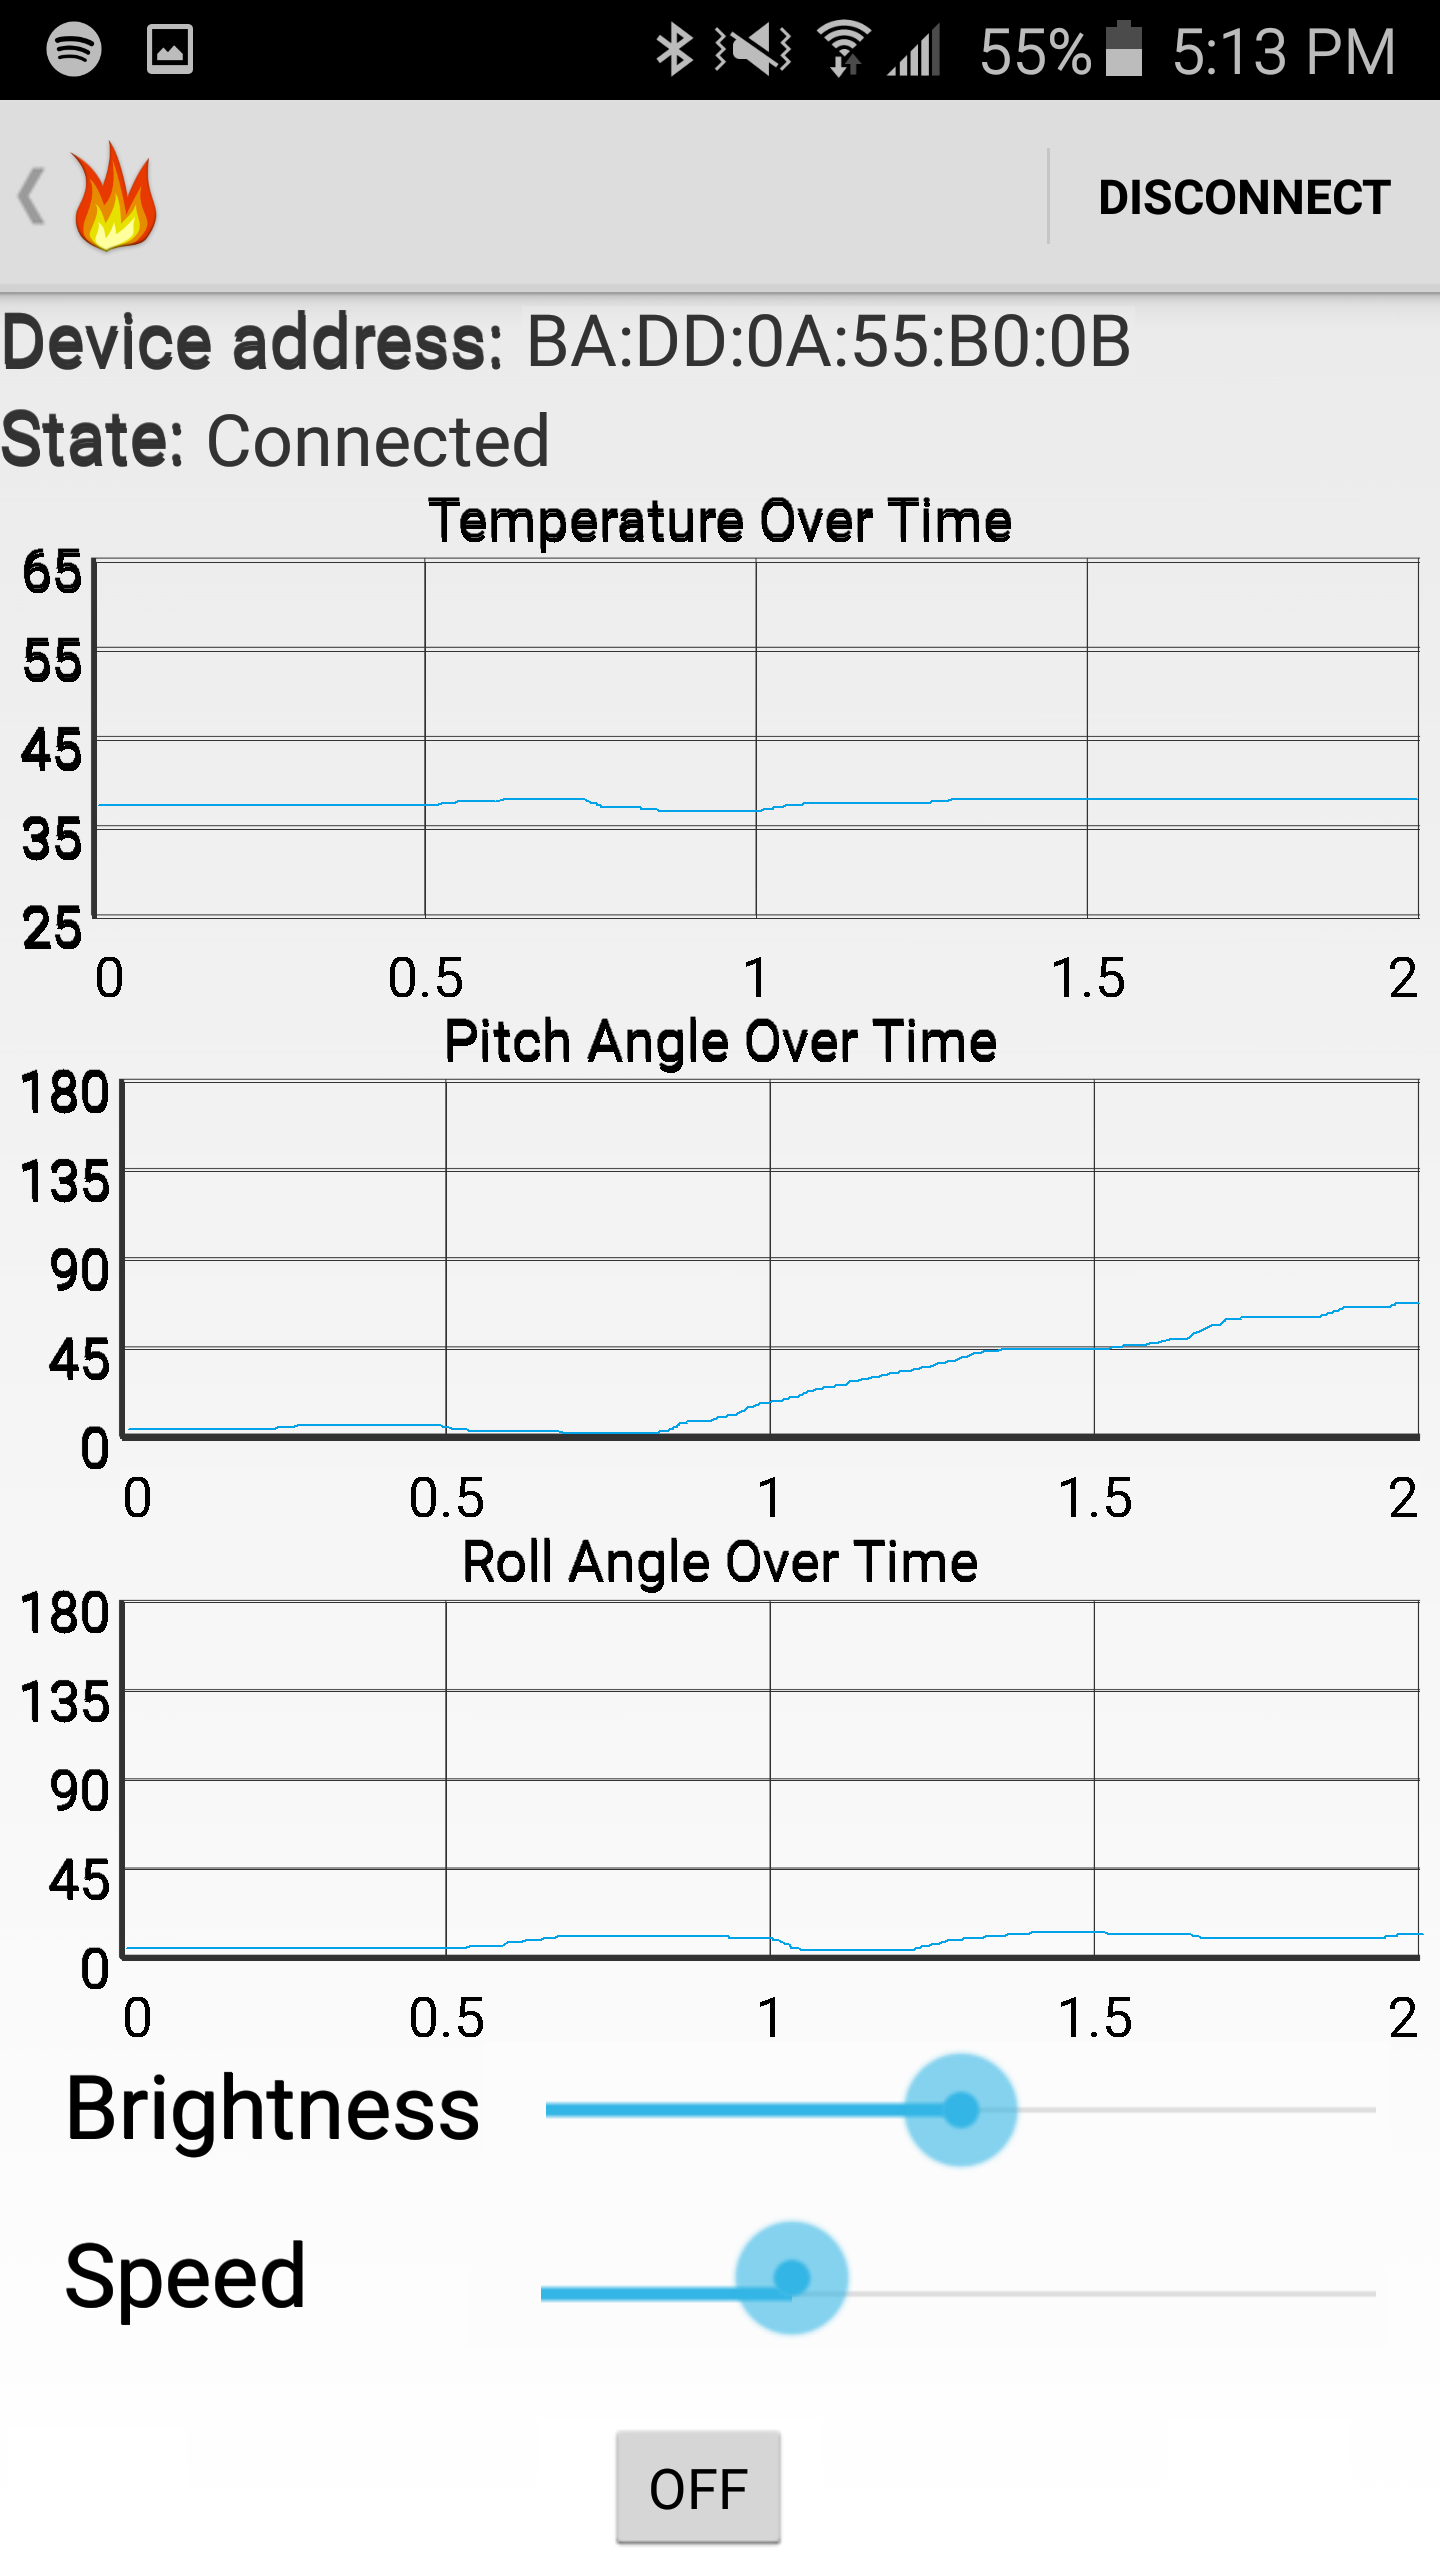
\includegraphics[scale=0.15]{images/android.png}
 \caption{Android Application Main View}
 \label{fig:android}
\end{figure}

First of all, the temperature, roll, and pitch data are presented to the user using graph from the Graph View library. For each of the values, a tread have been setup to read the Bluetooth characteristic and update the data points that are displayed on the graph every 20 milliseconds. The main thread would then update the view with the new data points.

Secondly, the view contains two sliders, which control the speed and brightness of the LEDs on the Discovery board. A listener has been instantiated for each of the sliders. When the user moves a slider the listener call a function that write the new value to the specific characteristic. The view also contains a button. When it is pressed the function that writes to the on/off characteristic is being called. This allows the user to change the state of the LEDs.

Lastly, when the double tap characteristic is being notified an Android notification is being displayed on the screen. If the phone is sleeping, the screen wakes up to display the notification.


\section{Testing and Observations}
\subsection{Double Tap}
First graphs of the raw acceleration value of when a double tap and other undesirable event happened were analysed ( figure \ref{fig:DTCAL1}, \ref{fig:DTCAL2}, \ref{fig:DTCAL3}). From these results, the filtering algorithm described above was implemented. The following observations guided the design of the algorithm:

\begin{figure}[!htb]
 \centering
 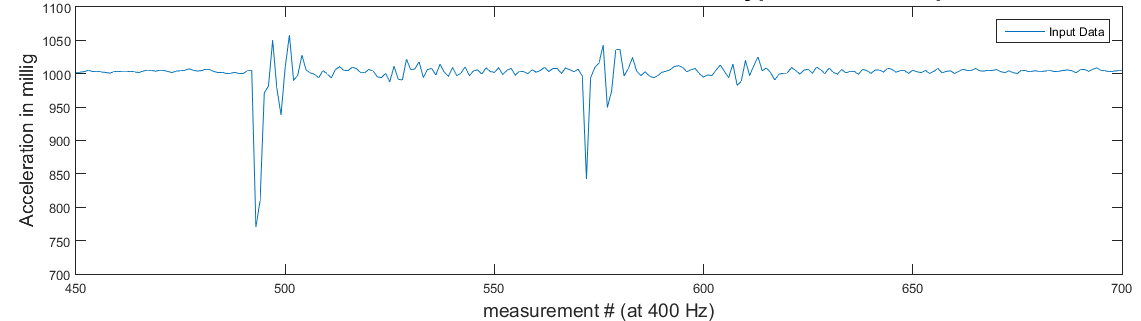
\includegraphics[scale=0.45]{images/DTcalibration1.png}
 \caption{Raw Acceleration Measurements from 3 Succesive Double Taps}
 \label{fig:DTCAL1}
\end{figure}

\begin{figure}[!htb]
 \centering
 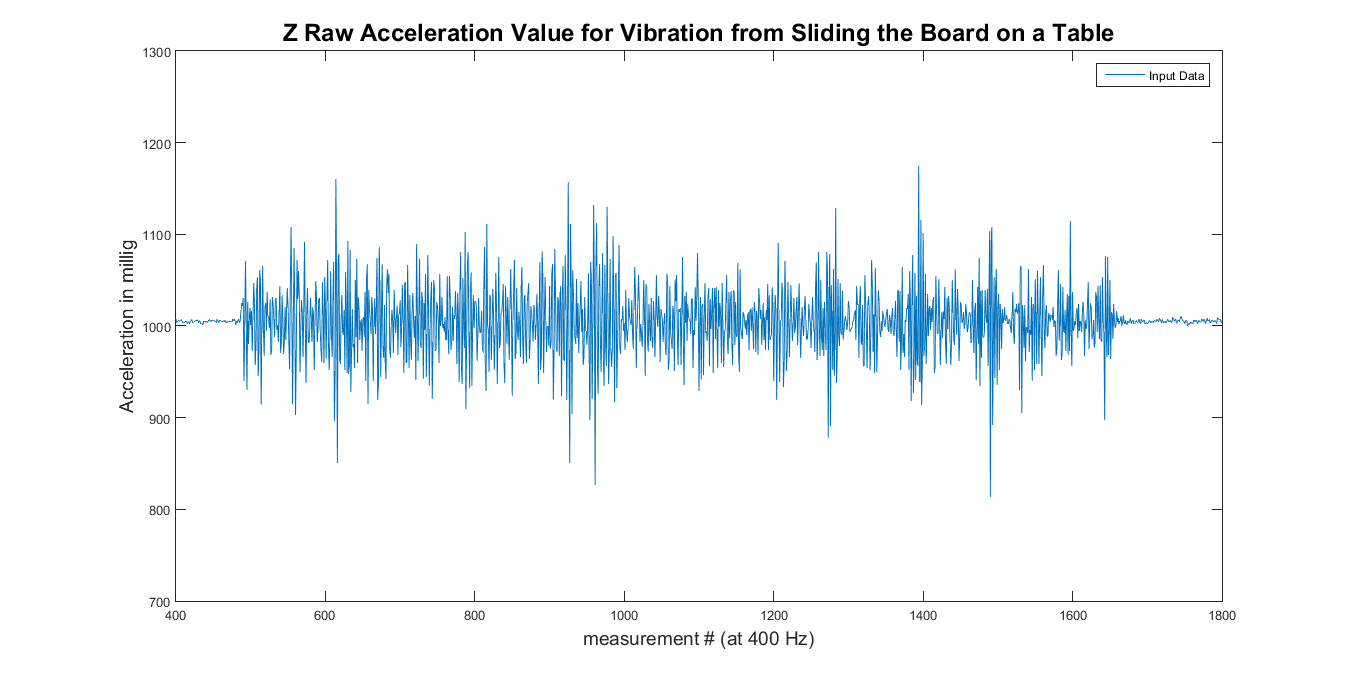
\includegraphics[scale=0.45]{images/DTcalibration2.png}
 \caption{Raw Acceleration Measurements from Sliding the Board on the Table}
 \label{fig:DTCAL2}
\end{figure}

\begin{figure}[!htb]
 \centering
 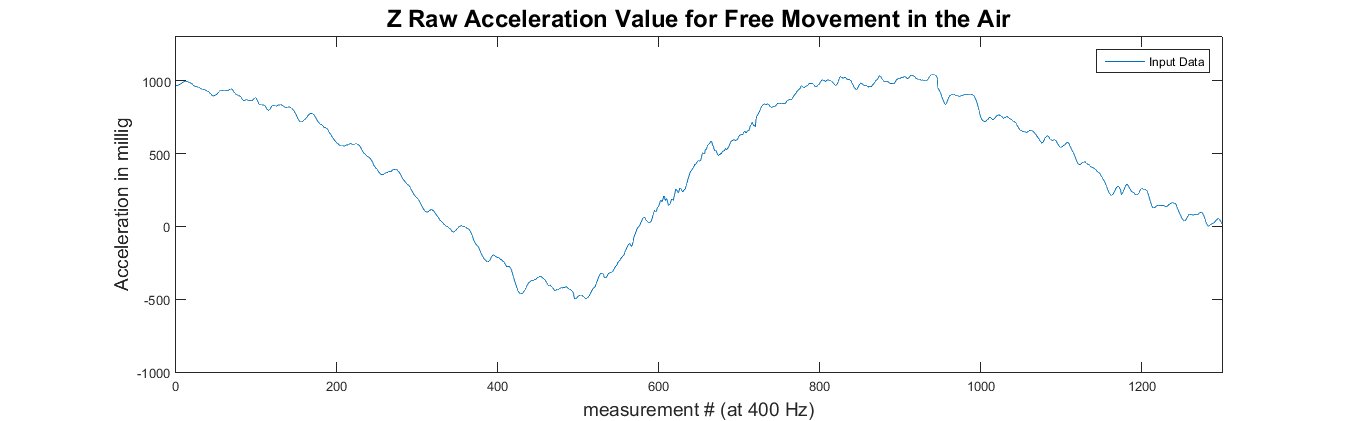
\includegraphics[scale=0.45]{images/DTcalibration3.png}
 \caption{Raw Acceleration Measurements from Free Movement in the Air}
 \label{fig:DTCAL3}
\end{figure}

\begin{itemize}
\item From figure \ref{fig:DTCAL1}, it was noted that a simple detection of a significant positive variation immediatly followed by a significant negative variation could be used to detect a spike. The polling frequency of the accelerometer had to be increased from 25 Hz to 400 Hz in order to capture all the spikes without fail.
\item From figure \ref{fig:DTCAL1} again, some ringing was noticed after a tap. To avoid detecting multiple spikes from one tap while maintaining a low threshold value for the amplitude of the spike, a delay where no spikes are detected was added. 
\item From figure \ref{fig:DTCAL3}, we can see that the variation when moving the board in the air is not as fast as a spike. Hence having a high frequency polling and a high enough amplitude can filter this out. 
\item From figure \ref{fig:DTCAL2}, we see that just sliding the board on the table generates multiple spikes. To make sure these vibrations would not trigger a double tap detection, a condition was implemented where if too much spikes were detected in the interval of time of the double tap, the double tap would not be counted.
\end{itemize}
After multiple hours of testing and adjusting of the parameter such as the amplitude and the time delays, a great DT detection algorithm was achieved. False positive from vibration and random movements for 5 minutes occured only twice.
 
\subsection{SPI}

\section{Timeline and Work Breakdown Between Team Members}
\begin{figure}[!htb]
 \centering
 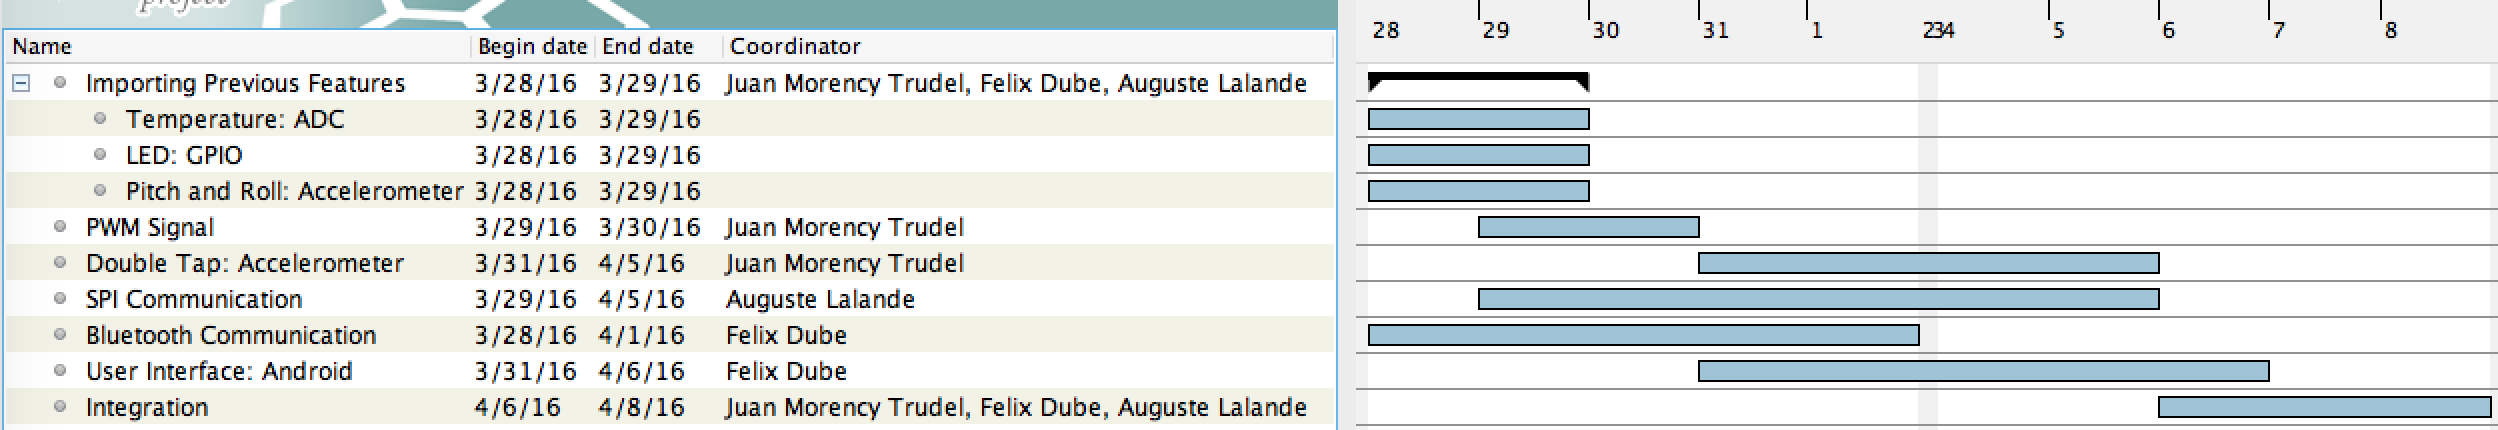
\includegraphics[scale=0.38]{images/gantt.png}
 \caption{Gantt Chart of the Project}
 \label{fig:Gantt}
\end{figure}
\section{Conclusion}

\newpage
\section{Bibliography}
\bibliographystyle{unsrt}
\bibliography{ProjectReport}

\newpage
\section{Appendix}
\begin{figure}[!htb]
 \centering
 \includegraphics[scale=0.6]{images/softwareArchitecture.png}
 \caption{High Level View of the Software Architecture}
 \label{fig:softArch}
\end{figure}


\begin{figure}[!htb]
 \centering
 \includegraphics[scale=0.50]{images/FSMDT.png}
 \caption{Finite State Machine of the Filtering Algorithm Required for Double Tap Detection}
 \label{fig:FSMDT}
\end{figure}


\end{document}
